
\begin{figure}[H]
\centering
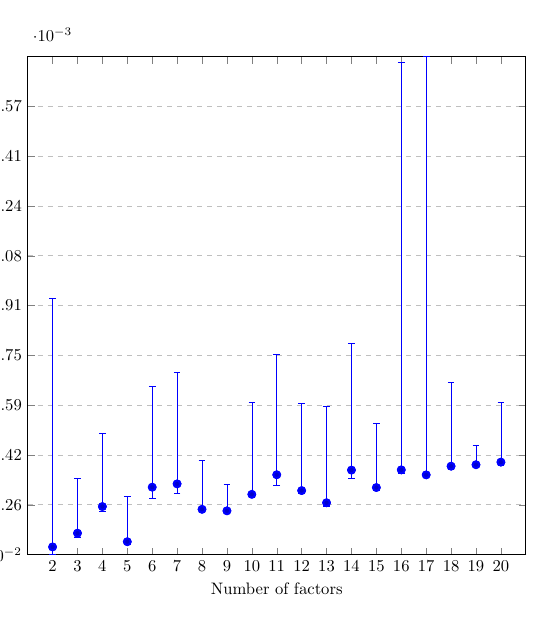
\begin{tikzpicture}[scale=0.6, trim axis left, trim axis right]
\begin{axis}[
    width=1\textwidth,
    height=1\textwidth,
    xlabel={Number of factors},
    ylabel={Time taken (s)},
    xmin=1.0, xmax=21.0,
    ymin=9.4e-05, ymax=0.001735,
    xticklabels={2, 3, 4, 5, 6, 7, 8, 9, 10, 11, 12, 13, 14, 15, 16, 17, 18, 19, 20},
    xtick={2, 3, 4, 5, 6, 7, 8, 9, 10, 11, 12, 13, 14, 15, 16, 17, 18, 19, 20},
    ytick={9.4e-05, 0.0002581, 0.0004222, 0.0005863, 0.0007504, 0.0009145, 0.0010786, 0.0012427, 0.0014068, 0.0015709},
    ymajorgrids=true,
    grid style=dashed,
]

\addplot+[
    blue,
    very thick,
    forget plot,
    only marks
    ]
    plot[
    very thick,
    error bars/.cd,
    y dir=plus,
    y explicit
    ]
    table[x=x,y=y,y error expr=\thisrow{y-max}] {
    x    y    y-max
    11	0.000356982894737	0.000398017105263
10	0.000292532894737	0.000304467105263
13	0.00026485	0.00031815
12	0.000304922368421	0.000287077631579
15	0.000314907894737	0.000210092105263
14	0.000372411842105	0.000418588157895
17	0.000356663157895	0.00137833684211
16	0.000373123684211	0.00134387631579
19	0.000390053947368	6.39460526316e-05
18	0.000385242105263	0.000274757894737
20	0.000398634210526	0.000197365789474
3	0.000164601315789	0.000180398684211
2	0.000119303947368	0.000819696052632
5	0.000136432894737	0.000150567105263
4	0.000252306578947	0.000239693421053
7	0.000327040789474	0.000365959210526
6	0.000316107894737	0.000332892105263
9	0.000238176315789	8.78236842105e-05
8	0.000243163157895	0.000161836842105

    };

\addplot+[
    blue,
    very thick,
    forget plot,
    only marks
    ]
    plot[
    very thick,
    error bars/.cd,
    y dir=plus,
    y explicit
    ]
    table[x=x,y=y,y error expr=\thisrow{y-min}] {
    x    y    y-min
    11	0.000356982894737	-3.39828947368e-05
10	0.000292532894737	-9.53289473685e-06
13	0.00026485	-1.185e-05
12	0.000304922368421	-9.92236842105e-06
15	0.000314907894737	-7.90789473684e-06
14	0.000372411842105	-2.64118421053e-05
17	0.000356663157895	-9.66315789473e-06
16	0.000373123684211	-1.21236842105e-05
19	0.000390053947368	-7.05394736842e-06
18	0.000385242105263	-9.24210526316e-06
20	0.000398634210526	-9.63421052632e-06
3	0.000164601315789	-1.46013157895e-05
2	0.000119303947368	-2.53039473684e-05
5	0.000136432894737	-8.43289473684e-06
4	0.000252306578947	-1.43065789474e-05
7	0.000327040789474	-3.00407894737e-05
6	0.000316107894737	-3.61078947368e-05
9	0.000238176315789	-6.17631578947e-06
8	0.000243163157895	-7.16315789474e-06

    };

\end{axis}
\end{tikzpicture}
\vspace{-0.3cm}
\caption{Small primes}\label{fig:TrialDivisionsmallprimesfactors}
\end{figure}
